\documentclass{article}
\usepackage{caption}
\usepackage{subcaption}
\usepackage{graphicx}
\usepackage{tikz}
\usepackage{tikzsymbols}
\usetikzlibrary{calc}
\usepackage{float}
\usepackage{pdflscape}
\usepackage{geometry}
\geometry{a4paper, landscape, margin=1cm}
\pagestyle{empty}

\def\centerarc[#1](#2)(#3:#4:#5){\draw[#1] ($(#2)+({#5*cos(#3)},{#5*sin(#3)})$) arc (#3:#4:#5);}

\begin{document}
	\centering
	\begin{figure}[H]
			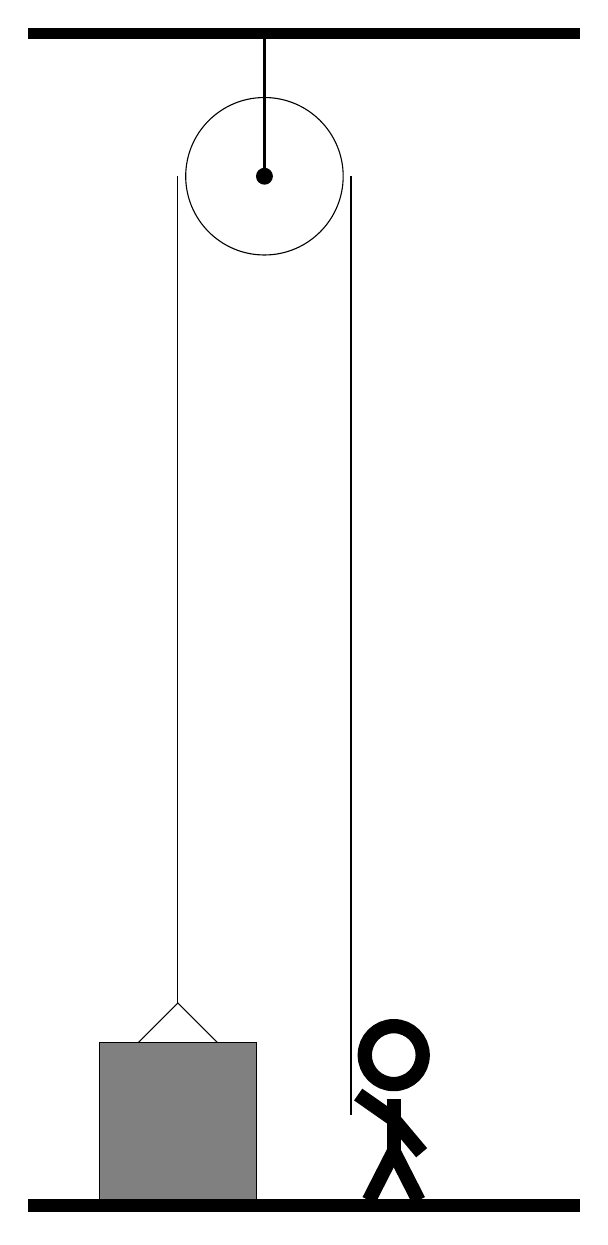
\begin{tikzpicture}
				%%%%% START %%%%%
								
				\draw[fill=black] (-2, 11.75) rectangle (5, 11.88);
				
				\draw (1, 10) circle (1);
				\draw[fill=black] (1, 10) circle (0.1);
				\draw[thick] (1, 11.75) -- (1, 10);
				
				\draw (-0.6, -1.0) -- (-0.1, -0.5) -- (0.4, -1.0);
				\draw[fill=black!50] (-1.1, -1.0) rectangle (0.9, -3.0);
				
				\draw (-0.1, 10) -- (-0.1, -0.5);
				\centerarc[thick](1, 10)(0:180:1.1);
				\draw[thick] (2.1, 10) -- (2.1, -1.92);
				
				\node at (2.6, -1.9) {\Strichmaxerl[10][-35][-50]};
				
				\draw[fill=black] (-2, -3) rectangle (5, -3.15);
				%%%%% END %%%%%
			\end{tikzpicture}
	\end{figure}	
\end{document}